\documentclass[border=10pt]{standalone}
\usepackage{pgfplots}
\pgfplotsset{compat=1.17}
\begin{document}
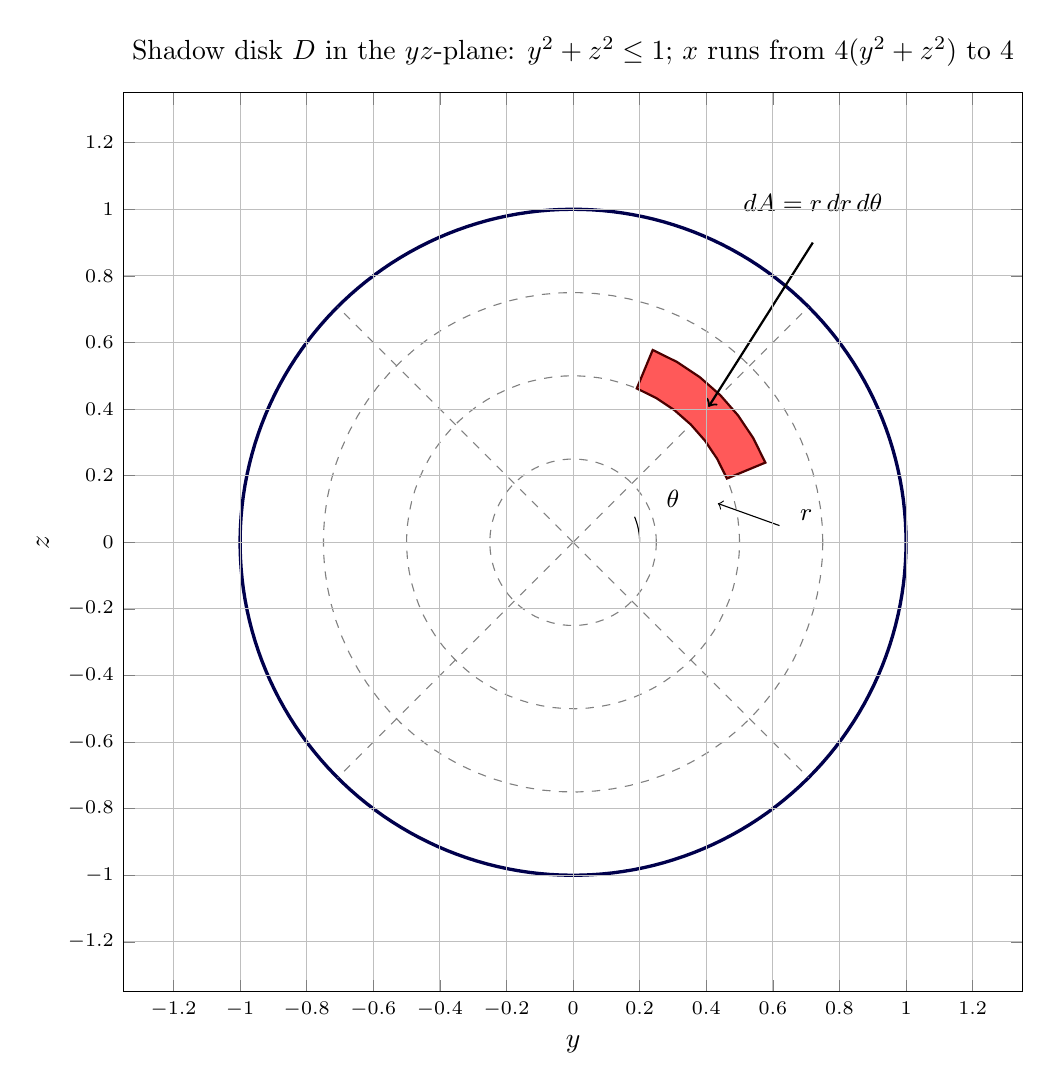
\begin{tikzpicture}
\begin{axis}[
    width=13cm, height=13cm,
    xlabel={$y$}, ylabel={$z$},
    xmin=-1.35, xmax=1.35, ymin=-1.35, ymax=1.35,
    axis equal image, grid=major, axis on top,
    title={Shadow disk $D$ in the $yz$-plane: $y^2+z^2\le 1$;  $x$ runs from $4(y^2+z^2)$ to $4$},
    tick label style={font=\scriptsize},
]
% boundary circle r = 1
\addplot[blue!30!black, very thick, domain=0:360, samples=200] ({cos(x)}, {sin(x)});
% polar grid: circles
\foreach \r in {0.25, 0.5, 0.75}
    \addplot[gray, dashed, thin, domain=0:360, samples=90] ({\r*cos(x)}, {\r*sin(x)});
% polar grid: rays
\foreach \a in {0, 45, ..., 315}
    \addplot[gray, dashed, thin] coordinates {(0,0) ({cos(\a)},{sin(\a)})};
% shaded polar element: r in [0.5, 0.625], theta in [22.5deg, 67.5deg]
\addplot[fill=red!65, draw=red!30!black, thick] coordinates {
    (0.46194,0.19134) (0.43301,0.25) (0.39668,0.30438) (0.35355,0.35355)
    (0.30438,0.39668) (0.25,0.43301) (0.19134,0.46194)
    (0.23918,0.57743) (0.3125,0.54127) (0.38048,0.49584) (0.44194,0.44194)
    (0.49584,0.38048) (0.54127,0.3125) (0.57743,0.23918)} -- cycle;
% annotation of dA
\draw[->, thick] (axis cs:0.72,0.9) -- (axis cs:0.40659,0.40659);
\node[font=\small] at (axis cs:0.72,1.02) {$dA = r\,dr\,d\theta$};
% r and theta markers
\draw[->, thin] (axis cs:0.62,0.05) -- (axis cs:0.43467,0.11647);
\node[font=\small] at (axis cs:0.7,0.08) {$r$};
\draw[thin] (axis cs:0.2,0) arc[start angle=0, end angle=22.5, radius=0.2];
\node[font=\small] at (axis cs:0.3,0.13) {$\theta$};
% axes through origin
\addplot[black, thin] coordinates {(-1.35,0) (1.35,0)};
\addplot[black, thin] coordinates {(0,-1.35) (0,1.35)};
\end{axis}
\end{tikzpicture}
\end{document}